\section{AddToSystem} \label{sec:AddToSystem}

This utility takes an existing system (or an empty system, i.e., creates new
system from scratch) and adds new beads (read from a \field file) into it,
placing them either completely randomly or according to supplied constraints.

There are two types of constraints which can be combined: place new beads (i)
specified distance from other beads or (ii) in a specified interval in x-, y-,
and/or z-axis directions. In (i), options \tt{-ld} and/or \tt{-hd} specify the
distance; if present, these must be accompanied by \tt{-bt} or \tt{--bonded}
option. The new beads are then placed at least \tt{-ld <float>} and at most
\tt{-hd <float>} distance from beads specified by the \tt{-bt} option or from
any bonded bead (\tt{--bonded} option).

In (ii), options \tt{-cx}, \tt{-cy}, and \tt{-cz} basically change the box size
for the added beads. By default, this constraint is specified in units relative
to the box dimensions (i.e., allowed values go from 0 to 1); use the \tt{--real}
option for absolute units. For example, \tt{-cx 0.5 1} would generate x
coordinates between 50\% and 100\% of the box's x sidelength.

All these options can be combined, but note that \tt{AddToSystem} does not
perform any sanity checks; that is, if any combination of the provided options
is impossible to achieve, the utility may run forever. See
\cref{fig:AddToSystem} for schematic examples.

\begin{figure}[b]
  \centering
  \begin{subfigure}{0.20\textwidth}
    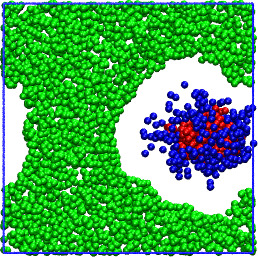
\includegraphics[height=0.9\textwidth]{AddToSystem-A-ld.jpg}
    \caption{}
  \end{subfigure}
  \hspace{15pt}
  \begin{subfigure}{0.20\textwidth}
    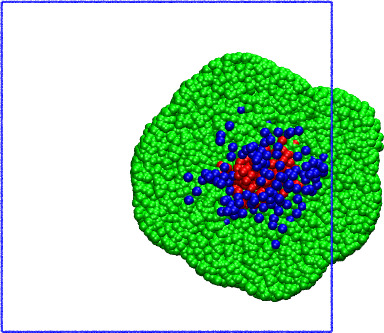
\includegraphics[height=0.9\textwidth]{AddToSystem-A-hd.jpg}
    \caption{}
  \end{subfigure}
  \hspace{15pt}
  \begin{subfigure}{0.20\textwidth}
    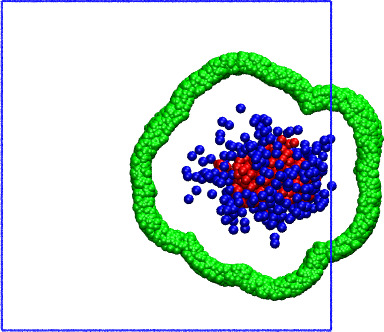
\includegraphics[height=0.9\textwidth]{AddToSystem-A-ld_hd.jpg}
    \caption{}
  \end{subfigure}

  \begin{subfigure}{0.20\textwidth}
    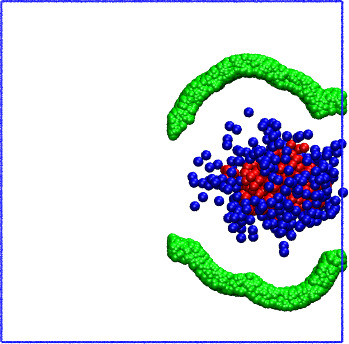
\includegraphics[height=0.9\textwidth]{AddToSystem-A-ld_hd_cx.jpg}
    \caption{}
  \end{subfigure}
  \hspace{15pt}
  \begin{subfigure}{0.20\textwidth}
    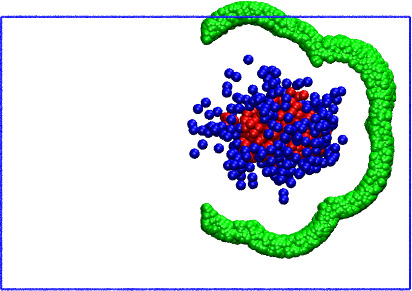
\includegraphics[width=1.0\textwidth]{AddToSystem-A-ld_hd_cx_b.jpg}
    \caption{}
  \end{subfigure}
  \hspace{15pt}
  \begin{subfigure}{0.20\textwidth}
    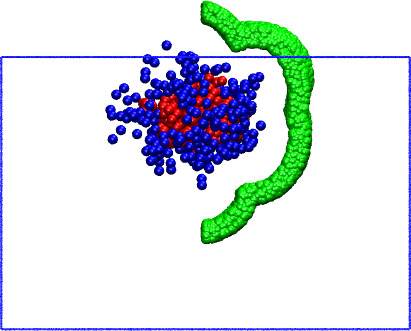
\includegraphics[width=1.0\textwidth]{AddToSystem-A-ld_hd_cx_b_off.jpg}
    \caption{}
  \end{subfigure}
  \caption{
    Examples of distance checks (cross-section snapshots): (a) \tt{-ld 3 -bt A
    B} specifies that any added bead (green) is at least at a distance of three
    from any \tt{A} or \tt{B} bead (red and blue, respectively); (b) \tt{-hd 4
    -bt A B} specifies added beads are at most four units away from any \tt{A}
    or \tt{B} bead; (c) combines (a) and (b) into \tt{-ld 3 -hd 4 -bt A B}, that
    is, new beads are added at a distance between three and four from any \tt{A}
    or \tt{B} bead; (d) combines (c) with axis constraint into \tt{-ld 3 -hd 4
    -cx 0.5 1 -bt A B} which constrains the x-coordinate of new beads between
    50\% and 100\% of the box's x sidelength; (e) adds \tt{-b 30 20 25} to the
    options in (d), changing the box size; finally, (f) also moves the original
    system, adding \tt{-off -0.2 0.2 0}. See \tt{Examples/AddToSystem/Manual}
    folder for source of these examples.
  }\label{fig:AddToSystem}
\end{figure}

For added molecules, either the molecule's geometric centre (default behaviour)
or its first bead (\tt{--head} option) obey these constraints. The coordinates
of the remaining beads in the molecule are governed by the coordinates in the
input \tt{FIELD} file. Therefore, not all the molecular beads necessarily obey
the constraining rules.

By default, molecules are added with a random orientation; when \tt{--no-rotate}
switch is used, the molecules are not rotated, but when \tt{-a} option is used,
all the molecules are rotated by the three angles specified in degrees.

The $\alpha$, $\beta$, and $\gamma$ angles in \tt{-a <alpha> <beta> <gamma>}
represent yaw, pitch, and roll, respectively. To put it in other words, it is an
intrinsic rotation with Tait-Bryan angles $\alpha$, $\beta$, and $\gamma$ about
axes $x$, $y$, and $z$, respectively. The rotation matrix, $R$, is, therefore,
defined as
\begin{equation}
  \begin{aligned}
  R &= R_z(\alpha) R_y(\beta) R_x(\gamma)\\
    &= \left[
    \begin{array}{ccc}
      \cos\alpha & -\sin\alpha & 0\\
      \sin\alpha &  \cos\alpha & 0\\
      0          & 0           & 1\\
    \end{array} \right]
    \left[
    \begin{array}{ccc}
      \cos\beta  & 0           & \sin\beta\\
      0          & 1           & 0\\
      -\sin\beta & 0           & \cos\beta\\
    \end{array} \right]
    \left[
    \begin{array}{ccc}
      1          & 0           & 0\\
      0          & \cos\gamma  & -\sin\gamma\\
      0          & \sin\gamma  & \cos\gamma\\
    \end{array} \right]\\
    &= \left[
    \begin{array}{ccc}
      \cos\alpha\cos\beta &
        \cos\alpha \sin\beta \sin\gamma - \sin\alpha \cos\gamma &
        \cos\alpha \sin\beta \cos\gamma + \sin\alpha \sin\gamma \\
      \sin\alpha\cos\beta &
        \sin\alpha \sin\beta \sin\gamma + \cos\alpha \cos\gamma &
        \sin\alpha \sin\beta \cos\gamma - \cos\alpha \sin\gamma \\
      -\sin\beta & \cos\beta \sin\gamma & \cos\beta \cos\gamma \\
    \end{array} \right]
  \end{aligned}
\end{equation}

By default, the new beads are exchanged for beads in the original system; what
bead type to exchange is either the most numerous one (default behaviour) or
provided via the \tt{-xb} option. Note that the utility doesn't check whether
exchanged beads are in a molecule, so a bonded bead may be exchanged, leaving
only part of the molecule in the new system. If beads are to be added into the
system rather than switched, use the \tt{--add} option.

The size of the new simulation box can be changed using the \tt{-b} option (the
new size must be in absolute units, i.e., it is unaffected by the \tt{--real}
option). Any constraints for placing beads are applied to this box rather than
the one in the original system. By default, the new system is placed so the
centres of the original box and the new one coincide. Note that periodic
boundary conditions are not applied to the new system, so the beads can be
outside the simulation box. If \tt{-off} option is used, the beads from the
input system are instead moved by the offset specified by the fraction of the
output simulation box (or in real units, if \tt{--real} is used) before the new
beads are added.

To create a new system instead of adding to an existing one, use \tt{-} instead
of an \tt{<input>} file. An extra file can be generated via the \tt{-o} option;
this can be useful to, e.g., generate both \vtf file for visualization and \data
file for use by LAMMPS.

Examples of using the utility (such as how to generate a bilayer or wire-like
aggregate) are provided in the \tt{Examples/AddToSystem} folder (including those
in \cref{fig:AddToSystem}).

\vspace{1em}
\noindent
Usage: \tt{AddToSystem <input.vcf> <out.vsf> <out.vcf> [options]}
\noindent
\begin{longtable}{p{0.235\textwidth}p{0.709\textwidth}}
  \toprule
  \multicolumn{2}{l}{Mandatory arguments}\\
  \midrule
  \tt{<input>/-}  & input coordinate file (or create a system from scratch)\\
  \tt{<in.field>} & input \field structure file for the new system\\
  \tt{<output>}   & output coordinate file for the new system\\
  \toprule
  \multicolumn{2}{l}{options} \\
  \midrule
  \tt{-o <file>}           & extra structure file\\
  \tt{-ld <float>}         & lowest distance from beads specified by
                             \tt{-bt} option\\
  \tt{-hd <float>}         & highest distance from beads specified by
                             \tt{-bt} option\\
  \tt{-bt <name(s)>}       & bead types to use in conjunction with
                             \tt{-ld} and/or \tt{-hd} options\\
  \tt{--bonded}            & use bonded beads for the distance condition
                             (overwrites \tt{-bt} option)\\
  \tt{-xb <name>}          & specify bead type to exchange (default: most
                             numerous bead type)\\
  \tt{--add}               & replace original beads instead of increasing the
                             total number of beads\\
  \tt{--real}              & use real coordinates for -cx/-cy/-cz/-off options
                             instead of fractions of input box size\\
  \tt{--no-rotate}         & do not randomly rotate added molecules\\
  \tt{-a 3$\times$<angle>} & rotate all added by molecules along x-, y-,
                             and z-axis\\
  \tt{--head}              & use molecule's first bead for distance check
                             (default: molecule's geometric centre)\\
  \tt{-cx 2$\times$<float>}& constrain x coordinate to interval
                             $\langle num, num2)$ (units relative to box size)\\
  \tt{-cy 2$\times$<float>}& constrain y coordinate to interval
                             $\langle num, num2)$ (units relative to box size)\\
  \tt{-cz 2$\times$<float>}& constrain z coordinate to interval
                             $\langle num, num2)$ (units relative to box size)\\
  \tt{--real}              & use \enquote{real} units instead of relative ones
                             for \tt{-cx}/\tt{-cy}/\tt{-cz} options\\
  \tt{-b <x> <y> <z>}      & side lengths of the new simulation box\\
  \tt{-s <int>}            & seed for random number generator\\
  \midrule
  \multicolumn{2}{p{0.948\textwidth}}{\tt{-i},
                                      \tt{-st},
                                      \tt{--verbose},
                                      \tt{--silent},
                                      \tt{--help},
                                      \tt{--version}}\\
  \bottomrule
\end{longtable}
